%Styles
\tikzstyle{cog} = [draw=black, inner sep=0, minimum size = 0.2cm, circle, node distance=2cm, path picture={ 
      \filldraw[] (path picture bounding box.west) -- (path picture bounding box.east)-- (path picture bounding box.north east) -- (path picture bounding box.north) -- (path picture bounding box.south) -- (path picture bounding box.south west) -- cycle;}]
\tikzstyle{force}=[>=latex,draw=blue,fill=blue]
\tikzstyle{axis} =[dashed,gray,font=\small]
\tikzstyle{spring} = [black,decorate,decoration={snake,amplitude=3.5,segment length=10}]
\tikzstyle{cart} = [rectangle, inner sep=0,minimum height=0.8cm, minimum width=1cm, node distance=1.8cm, path picture={ 
      \draw[] ([yshift=0.12cm, xshift=0.3pt] path picture bounding box.south west) rectangle ([xshift=-0.3pt,yshift=-0.3pt] path picture bounding box.north east); 
      \draw[thick, fill=white] ([yshift=0.12cm, xshift=-0.2cm] path picture bounding box.south east) circle (0.1cm);
      \draw[thick,fill=white] ([yshift=0.12cm, xshift=0.2cm] path picture bounding box.south west) circle (0.1cm);
      }]

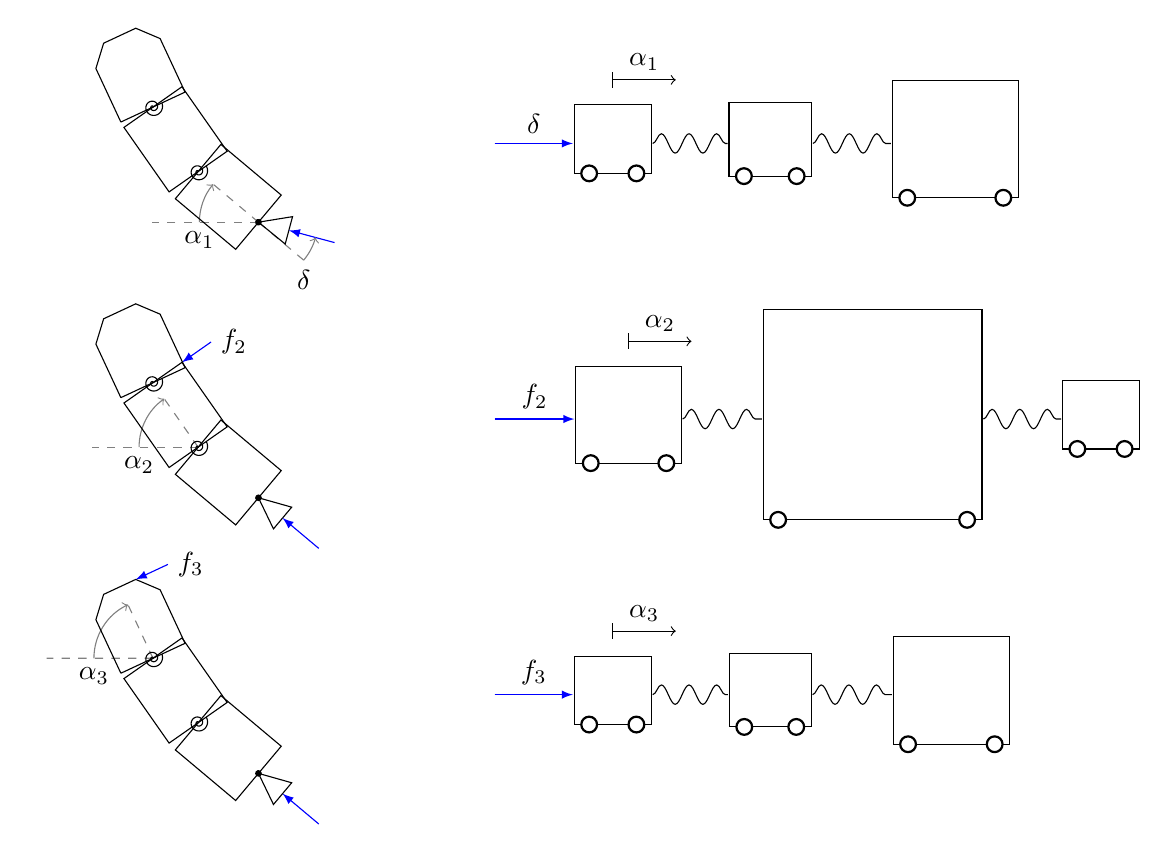
\begin{tikzpicture}[scale=1]

\def\h{1cm}
\def\w{0.9cm}
\def\thet{50}
\def\phio{-15}
\def\phit{-10}
\def\del{25}
\def\mw1{1cm}
\def\mh1{1cm}

	%%%%%%%%%%%%%%%%%%%%%%%%%%%%%%%%%%%%%%%%%%%%%%%%%%%%%%%%%%
 	\draw[axis]  (0,0) --  (-1.5*\w,0) node[left]{};
	\draw[draw=gray,->,] (-0.75*\h,0) node[below]{$\alpha_1$} arc (180:90+\thet:0.75*\h);
	
	\begin{scope}[yshift=0,rotate=\thet]
 	\draw[axis]  (0,-0.75*\h) -- (0,0)  node[above]{};
 	\draw[axis]  (0,0) -- (0,0.75*\h)  node[above]{};
	\draw[] (-\w/2,0) rectangle (\w/2,\h);
	
	\begin{scope}[yshift=\h,rotate=\phio]
	\draw[] (-\w/2,0) rectangle (\w/2,\h);
	\draw [domain=0:12.56,variable=\t,smooth,samples=75] plot ({\t r}: {0.010*\t});
	
	\begin{scope}[yshift=\h, rotate=\phit]
	\draw[] (-\w/2,0) -- (-\w/2,3*\h/4) -- (-\w/4,\h) -- (\w/4,\h) -- (\w/2,3*\h/4) -- (\w/2,0) --  (-\w/2,0) ;
	\draw [domain=0:12.56,variable=\t,smooth,samples=75] plot ({\t r}: {0.010*\t});
	
	\end{scope}
	\end{scope}
	
	\begin{scope}[rotate = \del]
	\draw[]  (0,0) -- (-0.2*\w,-0.4*\h) -- (0.2*\w,-0.4*\h) -- cycle;
	\draw[force,->] (0,-\h)  node[right]{}  -- (0,-0.4*\h);
	\filldraw (0,0) circle (1pt);
	\end{scope}
	\draw[draw=gray,->,] (0,-0.75*\h) node[below]{$\delta$} arc (-90:-90+\del:0.75*\h);
	\end{scope}

	\begin{scope}[xshift=3cm, yshift=1cm]
	\node[coordinate] (p) [] {};
	\node[cart,minimum width=1*\mw1, minimum height=1*\mh1]	(m1)		[right of=p, node distance=1.5cm]			{$$};
	\node[cart,minimum width=1.07*\mw1, minimum height=1.07*\mh1] 	(m2) 		[right of=m1, node distance=2cm] 	{$$};
	\node[cart,minimum width=1.62*\mw1, minimum height=1.62*\mh1] 	(m3) 		[right of=m2, node distance=2.35cm] 	{$$};
	 \draw[force,->] (p) -- node [above] {$\delta$} (m1);
	\draw[spring] (m1) -- node[above] {$$} (m2);
	\draw[spring] (m2) -- node[above] {$$} (m3);
	\draw ([yshift=0.4cm]m1.north) -- +(0,-0.2cm);
	\draw[->] ([yshift=0.3cm]m1.north) -- node[above] {$\alpha_1$} +(0.8cm,0);
	\end{scope}

	%%%%%%%%%%%%%%%%%%%%%%%%%%%%%%%%%%%%%%%%%%%%%%%%%%%%%%%%%
	\begin{scope}[yshift=-3.5cm,rotate=\thet]
	\draw[] (-\w/2,0) rectangle (\w/2,\h);
	
	\begin{scope}[yshift=\h,rotate=\phio]
	\begin{scope}[rotate=-\thet-\phio]
	\draw[axis]  (0,0) --  +(-1.5*\w,0) node[left]{};
	\draw[draw=gray,->,] (-0.75*\h,0) node[below]{$\alpha_2$} arc (180:90+\thet+\phio:0.75*\h);
	\end{scope}
	\draw[axis]  (0,0) -- (0,0.75*\h)  node[above]{};
	\draw[] (-\w/2,0) rectangle (\w/2,\h);
	\draw[force,->] (\w,\h)  node[right]{$f_2$}  -- (\w/2,\h);
	\draw [domain=0:12.56,variable=\t,smooth,samples=75] plot ({\t r}: {0.010*\t});

	\begin{scope}[yshift=\h, rotate=\phit]
	\draw[] (-\w/2,0) -- (-\w/2,3*\h/4) -- (-\w/4,\h) -- (\w/4,\h) -- (\w/2,3*\h/4) -- (\w/2,0) --  (-\w/2,0) ;
	\draw [domain=0:12.56,variable=\t,smooth,samples=75] plot ({\t r}: {0.010*\t});
	
	\end{scope}
	\end{scope}
	
	\begin{scope}[rotate = 0]
	\draw[]  (0,0) -- (-0.2*\w,-0.4*\h) -- (0.2*\w,-0.4*\h) -- cycle;
	\draw[force,->] (0,-\h)  node[right]{}  -- (0,-0.4*\h);
	\filldraw (0,0) circle (1pt);
	\end{scope}
	\end{scope}

	\begin{scope}[xshift=3cm, yshift=-2.5cm]
	\node[coordinate] (p) [] {};
	\node[cart,minimum width=1.36*\mw1, minimum height=1.36*\mh1]	(m1)		[right of=p, node distance=1.7cm]			{$$};
	\node[cart,minimum width=2.8*\mw1, minimum height=2.8*\mh1] 	(m2) 		[right of=m1, node distance=3.1cm] 	{$$};
	\node[cart,minimum width=1*\mw1, minimum height=1*\mh1] 	(m3) 		[right of=m2, node distance=2.9cm] 	{$$};
	\draw[force,->] (p) -- node [above] {$f_2$} (m1);
	\draw[spring] (m1) -- node[above] {$$} (m2);
	\draw[spring] (m2) -- node[above] {$$} (m3);
	\draw ([yshift=0.4cm]m1.north) -- +(0,-0.2cm);
	\draw[->] ([yshift=0.3cm]m1.north) -- node[above] {$\alpha_2$} +(0.8cm,0);
	\end{scope}
	
      %%%%%%%%%%%%%%%%%%%%%%%%%%%%%%%%%%%%%%%%%%%%%%%%%%%%%%%%%%%%%%%	
	\begin{scope}[yshift=-7cm,rotate=\thet]
	\draw[] (-\w/2,0) rectangle (\w/2,\h);

	\begin{scope}[yshift=\h,rotate=\phio]
	\draw[] (-\w/2,0) rectangle (\w/2,\h);
	\draw [domain=0:12.56,variable=\t,smooth,samples=75] plot ({\t r}: {0.010*\t});

	\begin{scope}[yshift=\h, rotate=\phit]
	\begin{scope}[rotate=-\thet-\phio-\phit]
	\draw[axis]  (0,0) --  +(-1.5*\w,0) node[left]{};
	\draw[draw=gray,->,] (-0.75*\h,0) node[below]{$\alpha_3$} arc (180:90+\thet+\phio+\phit:0.75*\h);
	\end{scope}
	 \draw[axis]  (0,0) -- (0,0.75*\h)  node[above]{};
	\draw[] (-\w/2,0) -- (-\w/2,3*\h/4) -- (-\w/4,\h) -- (\w/4,\h) -- (\w/2,3*\h/4) -- (\w/2,0) --  (-\w/2,0) ;
	\draw[force,->] (3*\w/4,\h)  node[right]{$f_3$}  -- (\w/4,\h);
	\draw [domain=0:12.56,variable=\t,smooth,samples=75] plot ({\t r}: {0.010*\t});
	
	\end{scope}
	\end{scope}
	
	\begin{scope}[rotate = 0]
	\draw[]  (0,0) -- (-0.2*\w,-0.4*\h) -- (0.2*\w,-0.4*\h) -- cycle;
	\draw[force,->] (0,-\h)  node[right]{}  -- (0,-0.4*\h);
	\filldraw (0,0) circle (1pt);
	\end{scope}
	\end{scope}
	
	\begin{scope}[xshift=3cm, yshift=-6cm]
	\node[coordinate] (p) [] {};
	\node[cart,minimum width=1*\mw1, minimum height=1*\mh1]	(m1)		[right of=p, node distance=1.5cm]			{$$};
	\node[cart,minimum width=1.06*\mw1, minimum height=1.06*\mh1] 	(m2) 		[right of=m1, node distance=2cm] 	{$$};
	\node[cart,minimum width=1.5*\mw1, minimum height=1.5*\mh1] 	(m3) 		[right of=m2, node distance=2.3cm] 	{$$};
	\draw[force,->] (p) -- node [above] {$f_3$} (m1);
	\draw[spring] (m1) -- node[above] {$$} (m2);
	\draw[spring] (m2) -- node[above] {$$} (m3);
	\draw ([yshift=0.4cm]m1.north) -- +(0,-0.2cm);
	\draw[->] ([yshift=0.3cm]m1.north) -- node[above] {$\alpha_3$} +(0.8cm,0);
	\end{scope}

\end{tikzpicture}